% Section 2: General-Form Prisoners' Dilemma Repeated
%-------------------------------------------------------------------------------

\begin{frame}{General Prisoners' Dilemma}
  \begin{table}[!h]
    \centering
    \begin{tabular}{*{4}{c|}}
      \multicolumn{2}{c}{} & \multicolumn{2}{c}{Column} \\ \cline{3-4}
      \multicolumn{1}{c}{} &         & Defect  & Cooperate \\ \cline{2-4}
      \multirow{2}*{Row} &    Defect & $D$,$D$ & $H$,$L$   \\ \cline{2-4}
                         & Cooperate & $L$,$H$ & $C$,$C$   \\ \cline{2-4} 
    \end{tabular} 
  \end{table} 

  What ordering of payoffs $D$, $H$, $L$, and $C$ make this a \textbf{Prisoners' Dilemma}? 
  \begin{enumerate}[label=\textbf{\alph*)}]
    \item $C > D > H > L$ 
    \item $H > D > C > L$ 
    \item $H > C > D > L$ 
    \item $C > H > L > D$
  \end{enumerate}
\end{frame}

\begin{frame}{General Prisoners' Dilemma}
  A single-stage prisoners' dilemma in extensive form:
  \usetikzlibrary{calc} 
  \begin{center}
  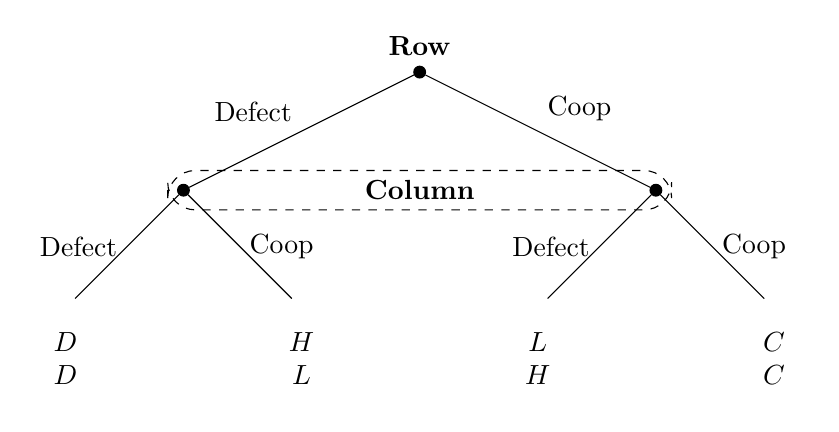
\begin{tikzpicture}
    \tikzstyle{solid node}=[circle,draw,inner sep=1.5,fill=black]
    \tikzstyle{level 1}=[level distance=15mm,sibling distance=6cm]
    \tikzstyle{level 2}=[level distance=15mm,sibling distance=3cm]
    \node(0)[solid node,label=above:{\textbf{Row}}]{}
        child{node(1)[solid node,label=above left:{}]{}
            child{node[label=below:{\begin{tabular}{c}
                    $D$ \\
                    $D$
                \end{tabular}}]{} edge from parent node[left]{Defect}}
            child{node[label=below:{\begin{tabular}{c}
                    $H$ \\
                    $L$
                \end{tabular}}]{} edge from parent node[right]{Coop}}
            edge from parent node[above left]{Defect}
        }
        child{node(2)[solid node,label=above right:{}]{}
            child{node[label=below:{\begin{tabular}{c}
                    $L$ \\
                    $H$
                \end{tabular}}]{} edge from parent node[left]{Defect}}
            child{node[label=below:{\begin{tabular}{c}
                    $C$ \\
                    $C$
                \end{tabular}}]{} edge from parent node[right]{Coop}}
            edge from parent node[above right]{Coop}
        };
    \draw[dashed,rounded corners=10]($(1) + (-.2,.25)$)rectangle($(2) +(.2,-.25)$);
    \node at($(1)!.5!(2)$){\textbf{Column}};
  \end{tikzpicture}
  \end{center}
\end{frame}

\begin{frame}{General Prisoners' Dilemma}
  A \textbf{two-stage} prisoners' dilemma in mixed extensive form:
  \usetikzlibrary{calc} 
  \begin{center}
    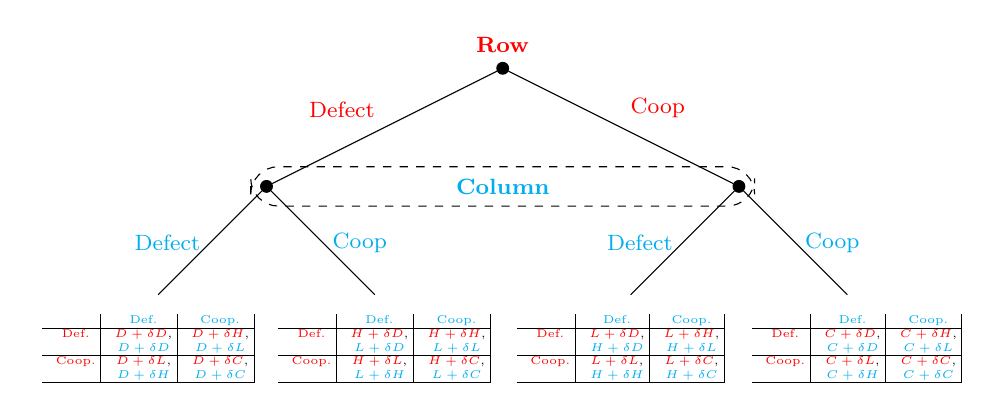
\begin{tikzpicture}[scale=1,font=\footnotesize]
    \tikzstyle{solid node}=[circle,draw,inner sep=1.5,fill=black]
    \tikzstyle{level 1}=[level distance=15mm,sibling distance=6cm]
    \tikzstyle{level 2}=[level distance=15mm,sibling distance=3cm]
    \node(0)[solid node,label=above:{\color{red} \textbf{Row}}]{}
      child{node(1)[solid node,label=above left:{}]{}
        child{node(3)[]{} edge from parent node[left]{\color{cyan}Defect}}
        child{node(4)[]{} edge from parent node[right]{\color{cyan}Coop}}
        edge from parent node[above left]{\color{red}Defect}
      }
      child{node(2)[solid node,label=above right:{}]{}
        child{node(5)[]{} edge from parent node[left]{\color{cyan}Defect}}
        child{node(6)[]{} edge from parent node[right]{\color{cyan}Coop}}
        edge from parent node[above right]{\color{red}Coop}
      };
    % info set
    \draw[dashed,rounded corners=10]($(1) + (-.2,.25)$)rectangle($(2) +(.2,-.25)$);
    \node at($(1)!.5!(2)$){\color{cyan} \textbf{Column}};
    % second stage
    \node[below] at(3){
      \tiny
      \scalebox{.82}{
      \begin{tabular}{*{3}{c<{\hspace{-4pt}}|}}
         & {\color{cyan} Def.} & {\color{cyan} Coop.} \\ \cline{1-3}
         {\color{red} Def.} & {\color{red} $D + \delta D$}, & {\color{red} $D + \delta H$},\\ 
                          & {\color{cyan}$D + \delta D$}  & {\color{cyan}$D + \delta L$} \\ \cline{1-3} 
         {\color{red} Coop.} & {\color{red} $D + \delta L$}, & {\color{red} $D + \delta C$},\\ 
                          & {\color{cyan}$D + \delta H$}  & {\color{cyan}$D + \delta C$} \\ \cline{1-3} 
      \end{tabular}
      }
    };
    \node[below] at(4){
      \tiny
      \scalebox{.82}{
      \begin{tabular}{*{3}{c<{\hspace{-4pt}}|}}
         & {\color{cyan} Def.} & {\color{cyan} Coop.} \\ \cline{1-3}
         {\color{red} Def.} & {\color{red} $H + \delta D$}, & {\color{red} $H + \delta H$},\\ 
                          & {\color{cyan}$L + \delta D$}  & {\color{cyan}$L + \delta L$} \\ \cline{1-3} 
         {\color{red} Coop.} & {\color{red} $H + \delta L$}, & {\color{red} $H + \delta C$},\\ 
                          & {\color{cyan}$L + \delta H$}  & {\color{cyan}$L + \delta C$} \\ \cline{1-3} 
      \end{tabular}
      }
    };
    \node[below] at(5){
      \tiny
      \scalebox{.82}{
      \begin{tabular}{*{3}{c<{\hspace{-4pt}}|}}
         & {\color{cyan} Def.} & {\color{cyan} Coop.} \\ \cline{1-3}
         {\color{red} Def.} & {\color{red} $L + \delta D$}, & {\color{red} $L + \delta H$},\\ 
                          & {\color{cyan}$H + \delta D$}  & {\color{cyan}$H + \delta L$} \\ \cline{1-3} 
         {\color{red} Coop.} & {\color{red} $L + \delta L$}, & {\color{red} $L + \delta C$},\\ 
                          & {\color{cyan}$H + \delta H$}  & {\color{cyan}$H + \delta C$} \\ \cline{1-3} 
      \end{tabular}
      }
    };
    \node[below] at(6){
      \tiny
      \scalebox{.82}{
      \begin{tabular}{*{3}{c<{\hspace{-4pt}}|}}
         & {\color{cyan} Def.} & {\color{cyan} Coop.} \\ \cline{1-3}
         {\color{red} Def.} & {\color{red} $C + \delta D$}, & {\color{red} $C + \delta H$},\\ 
                          & {\color{cyan}$C + \delta D$}  & {\color{cyan}$C + \delta L$} \\ \cline{1-3} 
         {\color{red} Coop.} & {\color{red} $C + \delta L$}, & {\color{red} $C + \delta C$},\\ 
                          & {\color{cyan}$C + \delta H$}  & {\color{cyan}$C + \delta C$} \\ \cline{1-3} 
      \end{tabular}
      }
    };
  \end{tikzpicture}
  \end{center} 
  Recall that $\delta$ is the subjective discount rate from stage to stage 
\end{frame}

\begin{frame}{Test Your Understanding}
  What should you do in the two-stage Prisoners' Dilemma 
  if your opponent plays \textit{Coop} in stage 1 and \textit{Coop} in stage 2?
  \begin{enumerate}[label=\textbf{\alph*)}]
    \item \textit{Coop} in stage 1, \textit{Coop} in stage 2
    \item \textit{Coop} in stage 1, \textit{Defect} in stage 2
    \item \textit{Defect} in stage 1, \textit{Coop} in stage 2
    \item \textit{Defect} in stage 1, \textit{Defect} in stage 2
  \end{enumerate}
\end{frame}

\begin{frame}{$\mathbb{T}$-stage repeated Prisoners' Dilemma}
  A complete strategy in a $\mathbb{T}$-stage repeated game will look like:
  \begin{align*}
    S_{t=1}^{\mathbb{T}} = 
    \begin{cases}
    \text{In stage } t=1 & \text{take action } A_0 \\ 
    \text{In stage } t>1 & 
    \begin{cases}
      \text{If history so far was } h_t, \text{take action } A_t(h_t) \\
      \text{Else if history was } h'_t, \text{take action } A_t(h'_t) \\ 
      ... 
    \end{cases}
    \end{cases}
  \end{align*}
  We can see that the number of possible strategies increases exponentially as $\mathbb{T}$ gets larger
\end{frame}

\begin{frame}{$\mathbb{T}$-stage repeated Prisoners' Dilemma}
  Suppose that $\mathbb{T}$ is a very large number, but we have played to the very last stage of a repeated Prisoners' Dilemma with that many stages:
  \begin{center}
    \begin{tabular}{*{4}{c|}}
      \multicolumn{2}{c}{} & \multicolumn{2}{c}{Column} \\ \cline{3-4}
      \multicolumn{1}{c}{} &        & Defect & Cooperate \\ \cline{2-4}
      \multirow{2}*{Row} & Defect   & Tot.$^R + D$, Tot.$^C + D$ & Tot.$^R + H$, Tot.$^C + L$ \\ \cline{2-4}
                         & Cooperate& Tot.$^R + L$, Tot.$^C + H$ & Tot.$^R + C$, Tot.$^C + C$ \\ \cline{2-4}
    \end{tabular} 
  \end{center}
  Let Tot.$^R$ and Tot.$^C$ represent the total payoffs that both players have earned over 
  stages 0 to $\mathbb{T} -1$
\end{frame}

\begin{frame}{$\mathbb{T}$-stage repeated Prisoners' Dilemma}
  \begin{center}
    \begin{tabular}{*{4}{c|}}
      \multicolumn{2}{c}{} & \multicolumn{2}{c}{Column} \\ \cline{3-4}
      \multicolumn{1}{c}{} &        & Defect & Cooperate \\ \cline{2-4}
      \multirow{2}*{Row} & Defect   & Tot.$^R + D$, Tot.$^C + D$ & Tot.$^R + H$, Tot.$^C + L$ \\ \cline{2-4}
                         & Cooperate& Tot.$^R + L$, Tot.$^C + H$ & Tot.$^R + C$, Tot.$^C + C$ \\ \cline{2-4}
    \end{tabular} 
  \end{center}
  Notice that the equilibrium of this subgame is still \textit{Defect}, \textit{Defect}
  because Tot.$^R$ and Tot.$^C$ are already decided by prior actions. 
\end{frame}

\begin{frame}{Repeated Prisoners' Dilemma with Uncertain Second Stage}
  Suppose that the first stage of the game is the Trenches Game:
  \begin{table}[!h]
    \centering
    \begin{tabular}{*{4}{c|}}
      \multicolumn{2}{c}{} & \multicolumn{2}{c}{German soldiers} \\ \cline{3-4}
      \multicolumn{1}{c}{} &    & Kill & Miss \\ \cline{2-4}
      \multirow{2}*{Allied Soldiers} & Kill & 4, 4 & 8, 2 \\ \cline{2-4}
                         & Miss & 2, 8 & 6, 6 \\ \cline{2-4} 
    \end{tabular} 
  \end{table}
  But with probability $p$, the game repeats in the second round 
  and with probability $1-p$, it ends after the first round
\end{frame}

\begin{frame}{Repeated Prisoners' Dilemma with Uncertain Second Stage}
  Consider the following strategy: 
  \begin{align*}
    \begin{cases}
      \text{In stage } 1 & : \textit{Miss} \\ 
      \text{In stage } 2 & : 
      \begin{cases}
        \textit{Miss} \text{  if the other player Missed in stage 1} \\ 
        \textit{Kill} \text{  if the other player Killed in stage 1}
      \end{cases}
    \end{cases}
  \end{align*}
  Let's call this strategy \textit{Punisher} because it starts off friendly, 
  but will try to punish someone who defects in the first round by defecting in the second round.
\end{frame}

\begin{frame}{Repeated Prisoners' Dilemma with Uncertain Second Stage}
  Suppose you are playing against a \textit{Punisher} in this game. 

  \begin{center}
    \begin{tabular}{*{4}{c|}}
      \multicolumn{2}{c}{} & \multicolumn{2}{c}{German soldiers} \\ \cline{3-4}
      \multicolumn{1}{c}{} &    & Kill & Miss \\ \cline{2-4}
      \multirow{2}*{Allied Soldiers} & Kill & 4, 4 & 8, 2 \\ \cline{2-4}
                         & Miss & 2, 8 & 6, 6 \\ \cline{2-4} 
    \end{tabular} 
  \end{center}

  \begin{itemize}
    \item What is your \textbf{expected utility} of playing \textit{Kill}, \textit{Kill}?
  \end{itemize}
  \vspace{10mm}
\end{frame}

\begin{frame}{Repeated Prisoners' Dilemma with Uncertain Second Stage}
  Suppose you are playing against a \textit{Punisher} in this game. 

  \begin{center}
    \begin{tabular}{*{4}{c|}}
      \multicolumn{2}{c}{} & \multicolumn{2}{c}{German soldiers} \\ \cline{3-4}
      \multicolumn{1}{c}{} &    & Kill & Miss \\ \cline{2-4}
      \multirow{2}*{Allied Soldiers} & Kill & 4, 4 & 8, 2 \\ \cline{2-4}
                         & Miss & 2, 8 & 6, 6 \\ \cline{2-4} 
    \end{tabular} 
  \end{center}

  What is your \textbf{expected utility} of playing \textit{Miss, Kill}? \\
  \vspace{10mm}
  What about from playing \textit{Kill, Miss?} \\
  \vspace{10mm}
  Would you rather defect earlier or later?
\end{frame}

\begin{frame}{Repeated Prisoners' Dilemma with Uncertain Second Stage}
  Suppose you are playing against a \textit{Punisher} in this game. 

  \begin{center}
    \begin{tabular}{*{4}{c|}}
      \multicolumn{2}{c}{} & \multicolumn{2}{c}{German soldiers} \\ \cline{3-4}
      \multicolumn{1}{c}{} &    & Kill & Miss \\ \cline{2-4}
      \multirow{2}*{Allied Soldiers} & Kill & 4, 4 & 8, 2 \\ \cline{2-4}
                         & Miss & 2, 8 & 6, 6 \\ \cline{2-4} 
    \end{tabular} 
  \end{center}

  What is your \textbf{expected utility} of playing \textit{Miss, Miss}?
  \vspace{10mm}
\end{frame}

\begin{frame}{Repeated Prisoners' Dilemma with Uncertain Second Stage}
  Let's graph your expected utilties of each strategy:
  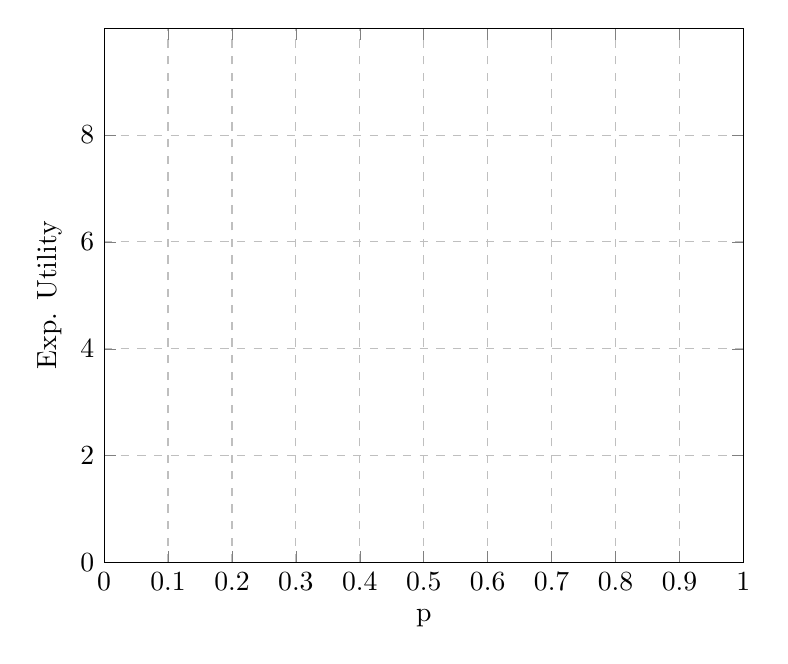
\begin{tikzpicture}
   \begin{axis}[
     width=0.8\textwidth,
     grid,
     xlabel={p},
     ylabel={Exp. Utility},
     xmin=0, xmax=1.0,
     ymin=0, ymax=10,
     xtick={0,.1,...,1.0},
     ytick={0, 2, 4, 6, 8},
     grid style=dashed,
     ]
 
     \addplot[draw=none] coordinates {(1,1)};
   \end{axis}
 \end{tikzpicture}
\end{frame}

\begin{frame}{Repeated Prisoners' Dilemma with Uncertain Second Stage}
  Now you should be getting some of the intuition for how cooperative equilibria might be achieved.
  \begin{itemize}
    \item We need the payoffs of the last period to be uncertain (or never reached)
    \item If trying to cheat a \textit{Punisher} or \textit{Grim Trigger} strategy, 
    it is better to start cheating them sooner rather than later
    \item In order for the equilibrium to have both players always cooperating,
    defecting in at least one period must not be a dominant strategy
  \end{itemize}
\end{frame}

\begin{frame}{Back to the General Form Prisoners' Dilemma}
  \begin{table}[!h]
    \centering
    \begin{tabular}{*{4}{c|}}
      \multicolumn{2}{c}{} & \multicolumn{2}{c}{Column} \\ \cline{3-4}
      \multicolumn{1}{c}{} &         & Defect  & Cooperate \\ \cline{2-4}
      \multirow{2}*{Row} &    Defect & $D$,$D$ & $H$,$L$   \\ \cline{2-4}
                         & Cooperate & $L$,$H$ & $C$,$C$   \\ \cline{2-4} 
    \end{tabular} 
  \end{table} 
  Now let's suppose that this game is repeated for an \textbf{infinite number of stages}.
\end{frame}

\begin{frame}{Extending Plays to Infinity}
  Suppose the game is in the `good' equilibrium where all players always play \textit{Cooperate}.
  \begin{itemize}
    \item What is \textbf{present value} from this equilibrium? 
    \begin{align*}
      pv\left(\{ C \}_{t=1}^{\infty}\right) & = C + \delta C + \delta^2 C + \delta^3 C + ... \\ 
         & = C \sum_{t=1}^{\infty} \delta^{t-1} \\
         & = C \frac{1}{1-\delta}
    \end{align*}
  \end{itemize}
\end{frame}

\begin{frame}{Extending Plays to Infinity}
   Let's extend the \textit{Punisher} strategy we had from the two-stage game 
   into the \textit{Grim Trigger strategy} of the general infinite horizon game:
  \begin{align*}
    \begin{cases}
      \text{In stage } 1 & : \textit{Cooperate} \\ 
      \text{In stage } t \geq 2 & : 
      \begin{cases}
        \textit{Cooperate} \text{  if only cooperation has happened so far} \\ 
        \textit{Defect} \text{  if anyone has \textit{ever} Defected in the past}
      \end{cases}
    \end{cases}
  \end{align*}
\end{frame}

\begin{frame}{Grim Trigger SPNE in Repeated PD}
  Is both players playing \textit{Grim Trigger} stable?
  \begin{itemize}
    \item Does a player have an incentive to \textit{Defect} against \texit{Grim Trigger}:
    \vspace{-5mm}
    \begin{align*}
      pv(Always~Coop) & \geq pv(Defect~once) \\
      C + \delta C + \delta^2 C + ...      & \geq H + \delta D + \delta^2 D + ...\\
      C + C \sum_{t=2}^{\infty} \delta^{t} & \geq H + D \sum_{t=2}^{\infty} \delta^{t} \\ 
      C + C \delta \sum_{t=2}^{\infty} \delta^{t-1} & \geq H + D \delta \sum_{t=2}^{\infty} \delta^{t-1} \\ 
      C + \frac{\delta C}{1 - \delta} & \geq H + \frac{\delta D}{1 - \delta} \\
      \delta & \geq \frac{H - C}{H - D}
    \end{align*}
  \end{itemize}
\end{frame}

\begin{frame}{Grim Trigger SPNE in Repeated PD}
  How do we interpret this statement:
  $$\text{Cooperation is stable when } \delta \geq \frac{H - C}{H - D}  $$ 
  \begin{itemize}
    \item Recall that the definition of the Prisoners' Dilemma was that $H > C > D > L$
    \item So this means $\frac{H - C}{H - D}$ is positive and less than 1 
    \item As the $H - C$, the relative benefit of defecting increases,
    it gets harder to sustain cooperation
    \item It also gets harder to sustain cooperation as the relative penalty of defecting, $H - D$, shrinks 
  \end{itemize}
\end{frame}

\begin{frame}{Other Strategies in Repeated Games}
  So far we've only looked at one example of a type of strategy in repeated game, 
  \textit{Grim Trigger}. 
  \begin{itemize}
    \item \underline{Can you think of some others?}
    \begin{itemize}
      \item Recall that a complete strategy for a repeated game needs: 
      \begin{itemize}
        \item An initial move at $t=1$
        \item A plan of action for \textit{every} possible history in \textit{every} later stage $t\geq2$
      \end{itemize}
      \item Ideally you would be able to tell a computer how to implement your strategy
    \end{itemize}
  \end{itemize}
\end{frame}

\begin{frame}{Other Strategies in Repeated Games}
  Telling a computer how to implement strategies is exactly what Robert Axelrod did in a famous tournament in 1980.
  \begin{itemize}
    \item He invited people to submit their programs which would play 200 rounds of the prisoners' dilemma against each other 
    \item The winning program was the one which had the highest total score after playing 200 rounds against all other programs
    \item What types of strategies do you think would succeed?
  \end{itemize}
\end{frame}

\begin{frame}{An Unexpected Winner}
  The winning program was named \texttt{TIT FOR TAT} \\ 
  Surprisingly, it was fairly simple:
  \begin{align*}
    \begin{cases}
      \text{In stage } 1 & : \textit{Cooperate} \\ 
      \text{In stage } t \geq 2 & : 
      \begin{cases}
        \text{repeat what the other player did in } t-1 \\
      \end{cases}
    \end{cases}
  \end{align*}
\end{frame}

\begin{frame}{Tit-for-Tat}
  Like \textit{Grim Trigger}, \textit{Tit-for-Tat} can punish other players for defecting. 
  \begin{itemize}
    \item If a player plays \textit{Defect}, it will copy them with \textit{Defect} next round 
  \end{itemize}
  But unlike \textit{Grim Trigger} it has a short memory; or is very forgiving
  \begin{itemize}
    \item If the player who defected goes back to playing cooperatively, 
    \textit{Tit-for-Tat} will go back to cooperating too
  \end{itemize}
\end{frame}

\begin{frame}{Axelrod's Tournament}
  If you want to learn more: 
  \begin{itemize}
    \item Read the original paper: 

    {
    \footnotesize
    Axelrod, Robert; Hamilton, William D. (27 March 1981), "The Evolution of Cooperation" (PDF), \textit{Science}, 211 (4489): 1390–96
    }

    \item The 1984 Book \textit{The Evolution of Cooperation}, Basic Books

    \item Run the tournament yourself in python!
    \url{https://github.com/Axelrod-Python/Axelrod}
    
    \item Play this fun and short web game! 
    \url{https://ncase.me/trust/}

  \end{itemize}
\end{frame}
